\section{RESULTADOS E DISCUSSÃO}
\label{sec:resultados}

Esta seção apresenta e discute os resultados dos dois estágios: o contexto do estado e a distribuição do IDEB, a segmentação socioeconômica, os fatores que diferenciam os municípios de alto e de baixo desempenho em cada grupo e, por fim, o diálogo com a literatura e as implicações para as políticas educacionais.

\subsection{Contexto socioeconômico e distribuição do IDEB}

No Censo Demográfico 2022, o Maranhão tem a menor renda domiciliar \textit{per capita} entre as 27 unidades da federação (R\$~899,87, contra R\$~1.638,06 no Brasil) \parencite{ibge2022} e a segunda maior proporção de moradores em pobreza extrema (26,6\%, contra 13,3\% no Brasil) \parencite{ibge2022classes}. A desigualdade entre os municípios também é expressiva: a renda \textit{per capita} mediana é de R\$~667, e a proporção de moradores em pobreza extrema varia de 11,2\% a 60,3\%.

A distribuição do IDEB dos 216 municípios com indicador divulgado é aproximadamente unimodal e ligeiramente assimétrica à direita, com média de 5,39 (desvio-padrão de 0,59), mediana de 5,30, mínimo de 4,10 e máximo de 8,10. A cauda superior é rarefeita: apenas 11 municípios atingem 6,50, e o máximo de 8,10 está um ponto acima do segundo maior valor (7,10). Ainda assim, a amplitude de 4,00 pontos, numa escala de 0 a 10, mostra que mesmo um estado vulnerável em termos nacionais tem variabilidade interna suficiente para justificar a investigação.

\subsection{Segmentação socioeconômica dos municípios}

Entre as partições testadas, de 2 a 10 grupos, o \textit{Silhouette Score} atinge o valor máximo em $k = 3$ (0,506), acima de $k = 2$ (0,489) e de $k = 4$ (0,456). A estabilidade \textit{bootstrap} confirma a escolha: o ARI médio é 0,812 em $k = 3$, contra 0,744 em $k = 2$ e 0,704 em $k = 4$. A partição com três grupos é, portanto, a mais bem separada e a mais estável sob reamostragem entre as testadas.

No gráfico~\ref{graf:pca}, os \textit{clusters} são projetados nas duas primeiras componentes principais. A primeira (PC1) explica 93,6\% da variância: os municípios se distribuem ao longo de um eixo de renda, em que renda média alta e pobreza extrema baixa caminham juntas.

\begin{grafico}[!ht]
  \centering
  \caption{Projeção dos \textit{clusters} de municípios maranhenses nas duas primeiras componentes principais para $k = 3$}
  \label{graf:pca}
  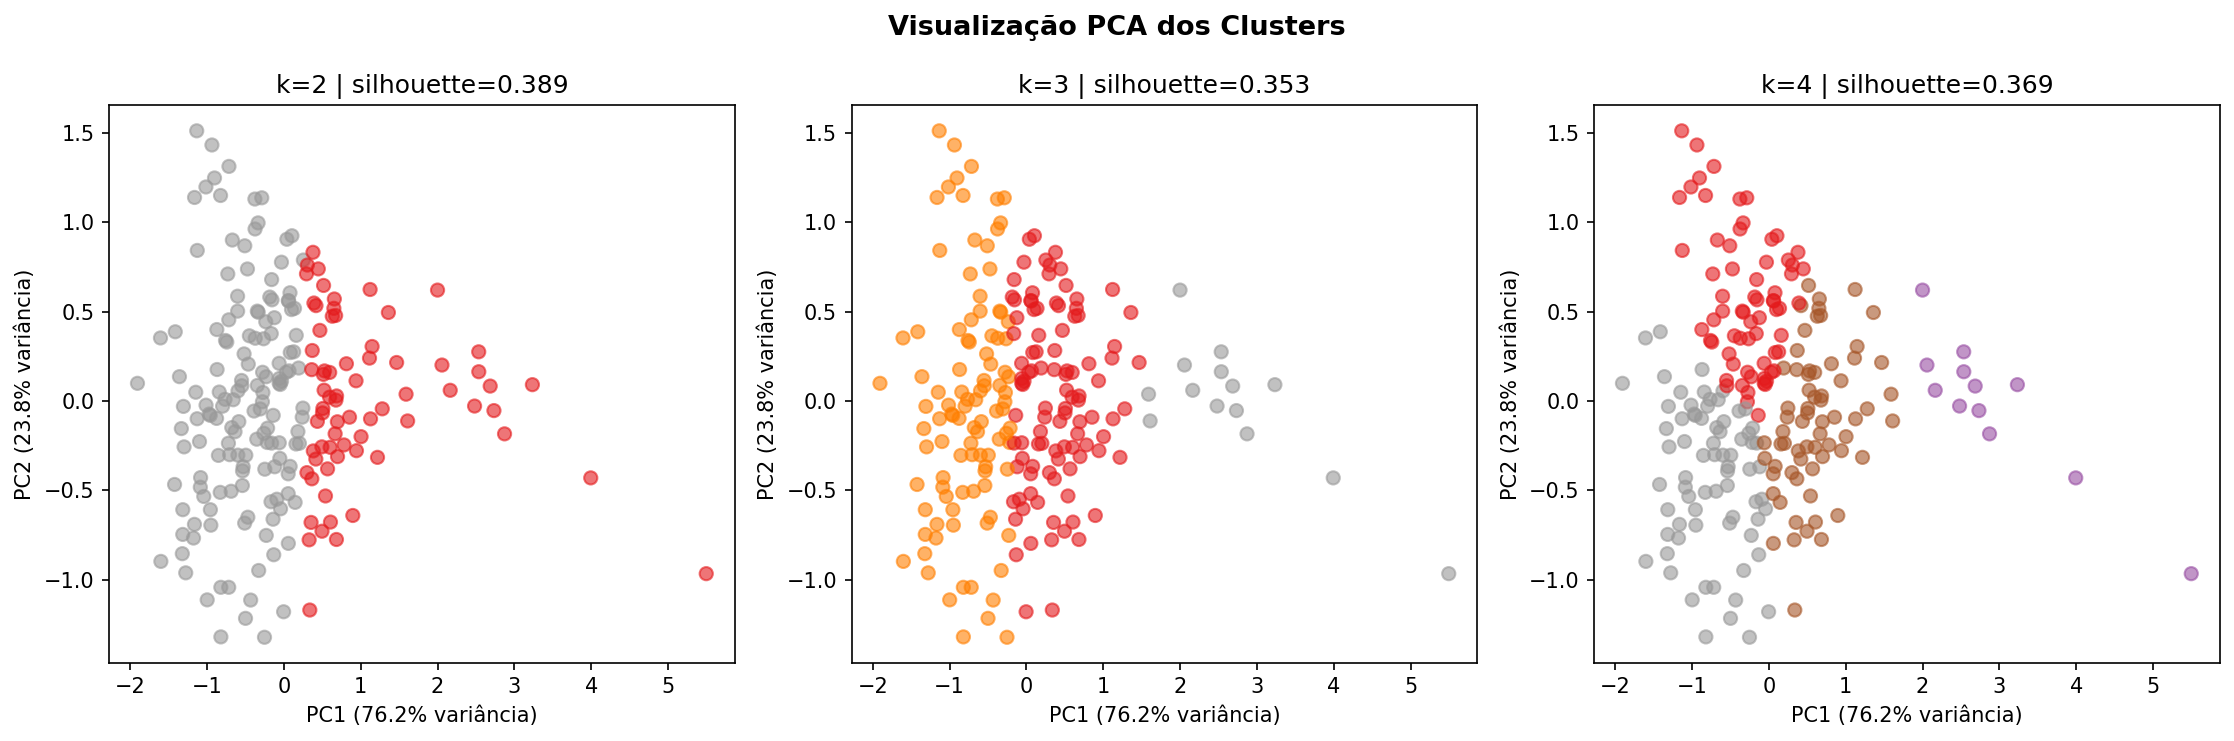
\includegraphics[width=0.72\textwidth]{pca_clusters.png}
  \fonte{elaboração própria com base em \textcite{ibge2022classes, ibge2022}.}
\end{grafico}

Na ablação, a concordância com a partição original cai para um ARI de 0,379 sem a renda \textit{per capita} e para 0,688 sem a pobreza extrema: as duas variáveis contribuem, com peso maior para a renda média.

O \textit{cluster} vulnerável (n = 88) tem renda \textit{per capita} média de R\$~555,84, 41,8\% dos moradores em pobreza extrema e IDEB médio de 5,29; o intermediário (n = 113), R\$~732,06, 27,5\% e 5,42; e o de alta renda (n = 15), R\$~1.082,44, 15,3\% e 5,78. Este último reúne a capital e os polos regionais, como Imperatriz, Timon e Balsas, e não tem amostra para a comparação por quartis, que deixaria quatro ou cinco municípios em cada extremo; a análise intragrupo concentra-se, assim, nos outros dois (201 municípios). A formação docente acompanha o gradiente de renda: 55,9\%, 64,0\% e 79,1\% dos docentes dos anos iniciais têm ensino superior nos três grupos.

\subsection{Fatores discriminantes no \textit{cluster} vulnerável}

Dentro do \textit{cluster} vulnerável (n = 88), os 24 municípios do quartil superior de IDEB (alto, $\geq 5{,}60$, média 6,08) são comparados aos 23 do quartil inferior (baixo, $\leq 4{,}80$, média 4,61). Na tabela~\ref{tab:mw}, apresentam-se as variáveis com $p < 0{,}10$ no teste de Mann-Whitney nos dois \textit{clusters}; as diferenças entre proporções são expressas em pontos percentuais (p.p.).

\begin{table}[!ht]
\centering
\caption{Variáveis com diferença entre municípios de alto e baixo IDEB nos \textit{clusters} vulnerável e intermediário (Mann-Whitney bicaudal)}
\label{tab:mw}
\corpodez
\setlength{\tabcolsep}{3pt}
\begin{tabular}{lcccccc}
\toprule
\textbf{Variável} & \textbf{Alto} & \textbf{Baixo} & \textbf{$\Delta$} & \textbf{$\delta$} & \textbf{$p$} & \textbf{$q$} \\
\midrule
\multicolumn{7}{l}{\textit{Cluster vulnerável (alto: n = 24; baixo: n = 23)}} \\
\% doc. com ensino superior & 60,6\% & 49,0\% & +11,6 p.p. & 0,35 & 0,039 & 0,34 \\
\% doc. com licenciatura     & 59,1\% & 47,8\% & +11,4 p.p. & 0,34 & 0,049 & 0,34 \\
\midrule
\multicolumn{7}{l}{\textit{Cluster intermediário (alto: n = 34; baixo: n = 29)}} \\
\% escolas com quadra                  & 12,9\%  & 5,4\%   & +7,5 p.p.  & 0,42 & 0,004 & 0,052 \\
\% turmas corr. fluxo (anos finais) & 0,90\%  & 0,07\%  & +0,8 p.p.  & 0,26 & 0,007 & 0,052 \\
\% doc. com ensino superior            & 69,2\%  & 58,1\%  & +11,1 p.p. & 0,29 & 0,047 & 0,18 \\
\% doc. com licenciatura               & 67,4\%  & 57,4\%  & +10,1 p.p. & 0,29 & 0,051 & 0,18 \\
Renda \textit{per capita} (R\$)        & 753,15  & 719,13  & +34,02     & 0,26 & 0,081 & 0,23 \\
\bottomrule
\end{tabular}
\nota{Alto e Baixo: médias dos grupos de alto e de baixo IDEB; $\Delta$: diferença entre as médias; $\delta$: delta de Cliff; $q$: valor $q$ de Benjamini-Hochberg sobre as catorze variáveis de cada \textit{cluster}.}
\fonte{elaboração própria com base em \textcite{inep2026microdados, inep2025, inep2026sinopse} e \textcite{ibge2022classes, ibge2022}.}
\end{table}

No \textit{cluster} vulnerável, só a formação docente diferencia os grupos: os municípios de IDEB alto têm 11,6 p.p. a mais de \textit{docentes com ensino superior} e 11,4 p.p. a mais com \textit{licenciatura}, com efeito médio ($\delta$ de 0,35 e 0,34). Esses testes não resistem à correção para comparações múltiplas ($q = 0{,}34$), mas a correlação de Spearman com os 88 municípios confirma a associação ($\rho = 0{,}29$ e $0{,}28$; $p \leq 0{,}009$; $q = 0{,}063$), e nenhuma outra variável se mantém após a correção ($q > 0{,}40$). Medida apenas na rede municipal, a associação fica mais forte ($\delta$ de 0,38 e 0,42; $p \leq 0{,}026$), de modo que a inclusão de docentes de outras redes na Sinopse não explica o resultado. Como quase todos os docentes com ensino superior são licenciados, as duas variáveis devem ser lidas como um único achado.

A renda \textit{per capita} e a pobreza extrema não diferenciam os grupos ($p = 0{,}322$ e $p = 0{,}463$), o que é compatível com o propósito da segmentação, embora a ausência de significância, com grupos de 23 e 24 municípios, não demonstre equivalência.

\subsection{Fatores discriminantes no \textit{cluster} intermediário}

Dentro do \textit{cluster} intermediário (n = 113), os 34 municípios do quartil superior de IDEB (alto, $\geq 5{,}70$, média 6,07) são comparados aos 29 do quartil inferior (baixo, $\leq 5{,}00$, média 4,81). As variáveis com $p < 0{,}10$ estão na segunda parte da tabela~\ref{tab:mw}.

A formação docente reaparece com magnitude semelhante: 11,1 p.p. a mais de \textit{docentes com ensino superior} e 10,1 p.p. a mais com \textit{licenciatura} nos municípios de IDEB alto ($\delta = 0{,}29$). A correlação de Spearman com os 113 municípios aponta na mesma direção ($\rho = 0{,}21$ e $0{,}20$; $p \leq 0{,}036$; $q \geq 0{,}12$), e a medida restrita à rede municipal reproduz o resultado ($\delta$ de 0,38 e 0,35; $p \leq 0{,}018$). Nenhum teste é conclusivo isoladamente; o que sustenta o achado é a repetição, com a mesma direção e magnitude, em dois grupos socioeconômicos e nos dois procedimentos de comparação.

A \textit{quadra esportiva} apresenta a diferença mais expressiva do \textit{cluster} ($p = 0{,}004$; $q = 0{,}052$; $\delta = 0{,}42$): a proporção de escolas com quadra é mais que o dobro nos municípios de IDEB alto, e a associação se mantém com todos os municípios do \textit{cluster} ($\rho = 0{,}23$; $q = 0{,}090$). Como a medida é municipal, o resultado não indica efeito da atividade esportiva sobre os alunos; a presença de quadras pode sinalizar um padrão mais amplo de investimento da rede em infraestrutura, leitura compatível com estudos que associam a infraestrutura ao IDEB nos anos iniciais \parencite{alves2013, vasconcelos2021}. A proporção de turmas de correção de fluxo nos anos finais também é maior nos municípios de IDEB alto ($p = 0{,}007$; $q = 0{,}052$), mas os valores são pequenos (menos de 1\% das turmas), o efeito é pequeno ($\delta = 0{,}26$), e não é possível inferir se a oferta de correção de fluxo é causa ou consequência do desempenho. A renda \textit{per capita} ainda difere marginalmente ($p = 0{,}081$), sinal de heterogeneidade residual de renda no maior \textit{cluster}.

\subsection{Diálogo com a literatura sobre o IDEB}

A centralidade da formação docente nos dois \textit{clusters} é compatível com a ênfase da literatura no papel do professor e com a prioridade que a política nacional atribui à licenciatura \parencite{brasil2014, gatti2019}. O estudo, porém, mede titulação no agregado municipal, e não qualidade docente, e \textcite{rivkin2005} e \textcite{glewwe2013} encontraram pouca relação entre titulação e aprendizado. Uma leitura possível é que, em redes nas quais mais de 40\% dos docentes ainda não concluíram a graduação, como as do \textit{cluster} vulnerável, a titulação diferencie os municípios mais do que em contextos em que ela já é quase universal. O resultado se enquadra na pesquisa em eficácia escolar \parencite{brooke2008} e na tese de \textcite{coleman1966}: controlado o contexto, que explica a maior parte da variação, as diferenças que restam entre redes se associam a fatores escolares de magnitude menor. O poder preditivo confirma essa leitura: o \textit{Random Forest} não separou os grupos de alto e de baixo IDEB melhor que o acaso (AUC de 0,51 no \textit{cluster} vulnerável e de 0,57 no intermediário), e a regressão \textit{ridge} não previu o IDEB melhor que a média ($R^2$ de $-0{,}01$ no estado, $-0{,}10$ e $-0{,}07$ nos \textit{clusters}). Os fatores identificados são, portanto, associações de magnitude modesta, e a maior parte da variação do IDEB depende de fatores que as bases administrativas não captam.

Quanto ao IDEB, a correlação entre fluxo e proficiência apontada por \textcite{soares2013} pede cautela, pois municípios podem priorizar a aprovação em detrimento da proficiência; como o índice incorpora a aprovação, as variáveis de fluxo guardam relação parcialmente mecânica com ele, o que pede a mesma cautela na leitura do achado sobre correção de fluxo.

\subsection{Implicações para as políticas educacionais}

A diferença na formação docente, repetida nos dois \textit{clusters}, torna a formação continuada e a indução à licenciatura candidatas plausíveis de política pública em todo o estado, e não apenas nos municípios mais pobres. A ampliação do Programa Nacional de Formação de Professores da Educação Básica (Parfor) pode ser considerada, com avaliação de impacto, já que a análise não quantifica o efeito esperado. No \textit{cluster} intermediário, a quadra esportiva indica a infraestrutura física complementar como candidata a priorização no monitoramento e na alocação orçamentária, embora a análise não permita estimar o retorno desse investimento.
